% This is a simple sample document.  For more complicated documents take a look in the exercise tab. Note that everything that comes after a % symbol is treated as comment and ignored when the code is compiled.

\documentclass{article} % \documentclass{} is the first command in any LaTeX code.  It is used to define what kind of document you are creating such as an article or a book, and begins the document preamble

\usepackage{amsmath} % \usepackage is a command that allows you to add functionality to your LaTeX code
\usepackage{tikz}
\usepackage{listings} %code extracts
\usepackage{xcolor} %custom colours
\usepackage{mdframed} %nice frames

\usetikzlibrary{arrows}

\title{Permutations} % Sets article title
\author{Claus Vind-Andreasen} % Sets authors name
\date{\today} % Sets date for date compiled

% The preamble ends with the command \begin{document}
\begin{document} % All begin commands must be paired with an end command somewhere
    \maketitle % creates title using information in preamble (title, author, date)
    
    \section{Introduction!} % creates a section
    
    \text
 This is a note documenting a mapping from n to a specific permuation of N items

  \section{Description  } % creates a section
    
We are here considering permuations of N objects. There are \(  N!  = N \times (N-1) \times (N-2) \times.......\times 3 \times 2 \times 1 \)  of these permutations 
\\
 ( for the first item you have N choices, for  the second item you have  N-1 choises and so on... ).
\\
\begin{enumerate}
\item
We have two bookcases, each with N shelves, the shelves  numbered from the bottom 0,1,2, .. to .N-1 (the topmost) .  
\item
The source bookcase has a box on each shelf, the destination bookcase has all shelves empty initially.  
\item
We will move boxes from the source bookcase to th destination bookcase following  the recipe  specified below, which tells us from  which shelf to take a box  in the source bookcase and where to put the box in the destination bookcase. 
\end{enumerate}
\noindent

It is obvious how to take a box from a non-empty shelf (and we will only be directed to do that), but putting a box on a shelf in the destination bookcase, has two variants.
\begin{enumerate}
\item 
the shelf is empty, we just put the box on the shelf
\item 
the shelf already contains a box, in this case all boxes on the  non-empty shelves from our destination shelf and upward  are  moved one shelf up, retaining their relative position.
\end{enumerate}
\newpage
\noindent 
The algorithm proceeds as follow:
 
\begin{enumerate}
\item 
We are given n, an integer, as the input
\item We count the number of non-empty shelves in the destination bookcase and call it X   (first time it is 0)
\item We calculate the position P as P = n modulo (X+1)
\item We take the topmost box in the Source bookcase and move it to the shelf with number P
\item  We change n to \( \lfloor n/( X+1)\rfloor  \), the integer part of  n divided by X+1
\item If the source bookcase is empty we are done, else we go back to step 2 and proceeds from there
\end{enumerate}
You will notice the mysterious X is just a counter going 0,1,2,3,4,5 with an increment for eaxh iteration of the loop (since the number of non-empty bookcases decrease by one each loop) . I used it to keep things simple, avoiding  a strange counter.
\\
\\
The input parameter n can be any integer, but the algorithm works on n modulo N!, so n = x gives the same permutation as \(n = x + N! \) or \( n =x +  2 \times N!\) or   \( n = x +  3  \times N!\) and so on....
\\
\\
\noindent Let us try this out for N = 4,
on the left we have our source book case, filled with 4 boxes  and on the right we have our destination book case, with empty shelves.  The shelves are numbered  0,1,2,3 from the bottom up.
\\
\\
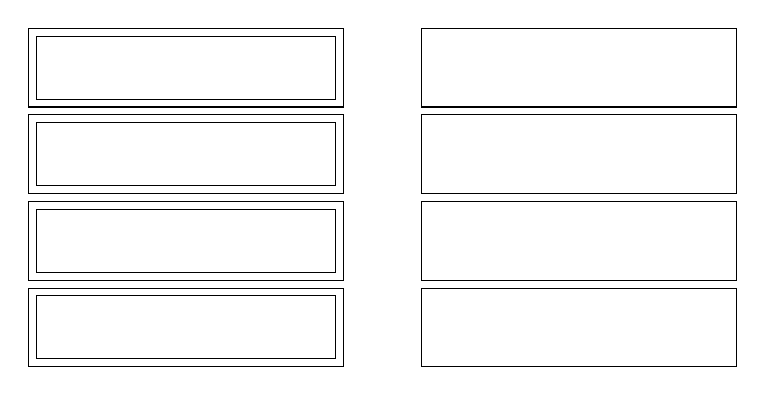
\begin{tikzpicture}
\draw (0,0) rectangle (4,1);
\draw (0.1,0.1) rectangle (3.9,0.9);
\draw (5,0) rectangle (9,1);
\draw (0, 1.1) rectangle (4,2.1);
\draw (0.1, 1.2) rectangle (3.9 ,2.0);

\draw (5, 1.1) rectangle (9,2.1);

\draw (0, 2.2) rectangle (4,3.2);
\draw (0.1, 2.3) rectangle (3.9,3.1);

\draw (5, 2.2) rectangle (9,3.2);

\draw (0, 3.3) rectangle (4,4.3);
\draw (0.1, 3.4) rectangle (3.9,4.2);

\draw (5, 3.3) rectangle (9,4.3);


\end{tikzpicture}
\\
\\
There are 4! = 24 different permutations, let's try to make permutation 17 = n 
\\
\\
The first move will take the top-most box (which we label "box A", to keep track of it)  on the source book case and move it to shelf 0 and n is unmodified.
\\
\\
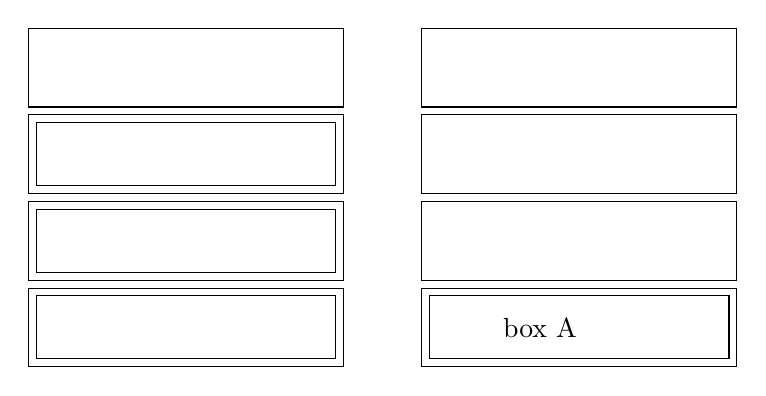
\begin{tikzpicture}
\draw (0,0) rectangle (4,1);
\draw (0.1,0.1) rectangle (3.9,0.9);
\draw (5,0) rectangle (9,1);
\draw (0, 1.1) rectangle (4,2.1);
\draw (0.1, 1.2) rectangle (3.9 ,2.0);

\draw (5, 1.1) rectangle (9,2.1);

\draw (0, 2.2) rectangle (4,3.2);
\draw (0.1, 2.3) rectangle (3.9,3.1);

\draw (5, 2.2) rectangle (9,3.2);

\draw (0, 3.3) rectangle (4,4.3);
%\draw (0.1, 3.4) rectangle (3.9,4.2);

\draw (5, 3.3) rectangle (9,4.3);
\draw (5.1, 0.1) rectangle (8.9,0.9);
%\node[draw] at (5.5, 0.5) {some text};
\node  at (6.5, 0.5) {box A};

\end{tikzpicture}
\\
\\
\noindent The second move will take the top-most box  (which we label "box B")  on the source book case and move it to shelf 1  ( = 17 mod2 ) and n is updated to  \( \lfloor 17/( 1+1)\rfloor   = 8 \),
\\
\\
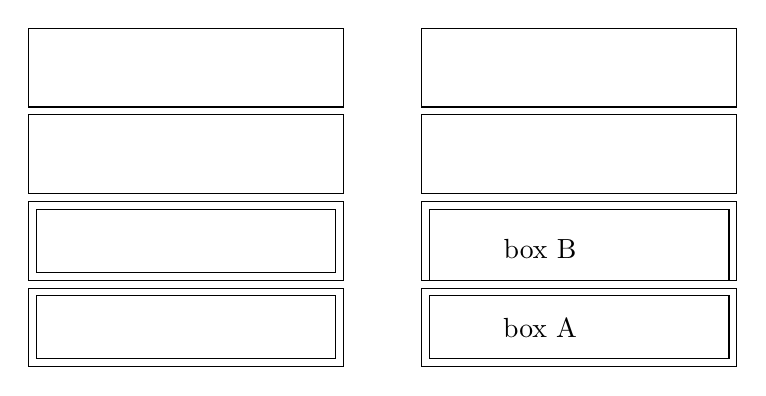
\begin{tikzpicture}
\draw (0,0) rectangle (4,1);
\draw (0.1,0.1) rectangle (3.9,0.9);
\draw (5,0) rectangle (9,1);
\draw (0, 1.1) rectangle (4,2.1);
\draw (0.1, 1.2) rectangle (3.9 ,2.0);

\draw (5, 1.1) rectangle (9,2.1);

\draw (0, 2.2) rectangle (4,3.2);
%\draw (0.1, 2.3) rectangle (3.9,3.1);

\draw (5, 2.2) rectangle (9,3.2);

\draw (0, 3.3) rectangle (4,4.3);
%\draw (0.1, 3.4) rectangle (3.9,4.2);

\draw (5, 3.3) rectangle (9,4.3);
\draw (5.1, 0.1) rectangle (8.9,0.9);
\draw (5.1, 1.1) rectangle (8.9,2.0);
\node  at (6.5, 0.5) {box A};
\node  at (6.5, 1.5) {box B};


\end{tikzpicture}
\\
\\
\noindent The third move will take the top-most box  (which we label "box C") on the source book case and move it to shelf 2  ( = 8 mod 3 ) and n is updated to  \( \lfloor 8/( 2+1)\rfloor   = 2 \),
\\
\\
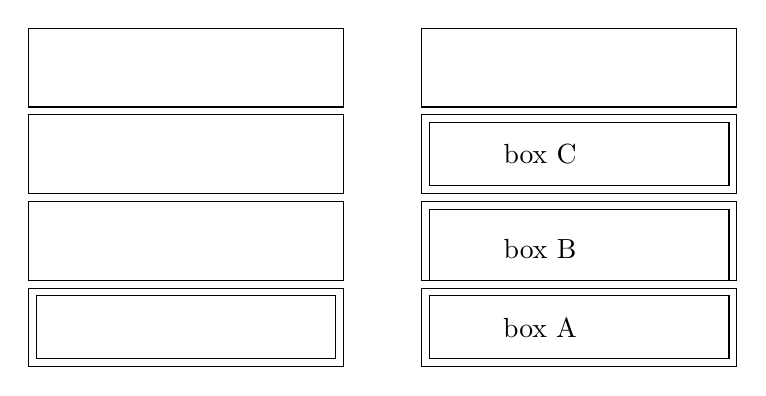
\begin{tikzpicture}
\draw (0,0) rectangle (4,1);
\draw (0.1,0.1) rectangle (3.9,0.9);
\draw (5,0) rectangle (9,1);
\draw (0, 1.1) rectangle (4,2.1);
%\draw (0.1, 1.2) rectangle (3.9 ,2.0);

\draw (5, 1.1) rectangle (9,2.1);

\draw (0, 2.2) rectangle (4,3.2);
%\draw (0.1, 2.3) rectangle (3.9,3.1);

\draw (5, 2.2) rectangle (9,3.2);

\draw (0, 3.3) rectangle (4,4.3);
%\draw (0.1, 3.4) rectangle (3.9,4.2);

\draw (5, 3.3) rectangle (9,4.3);
\draw (5.1, 0.1) rectangle (8.9,0.9);
\draw (5.1, 1.1) rectangle (8.9,2.0);
\draw (5.1, 2.3) rectangle (8.9,3.1);

\node  at (6.5, 0.5) {box A};
\node  at (6.5, 1.5) {box B};
\node  at (6.5, 2.7) {box C};


\end{tikzpicture}

\noindent The fourth move will take the top-most ( and last )  box  ( which we label "box D") on the source book case and move it to shelf 2 ( = 2 mod (3+1) ) and n is set to 0 ´, since we are done.
\\
\\
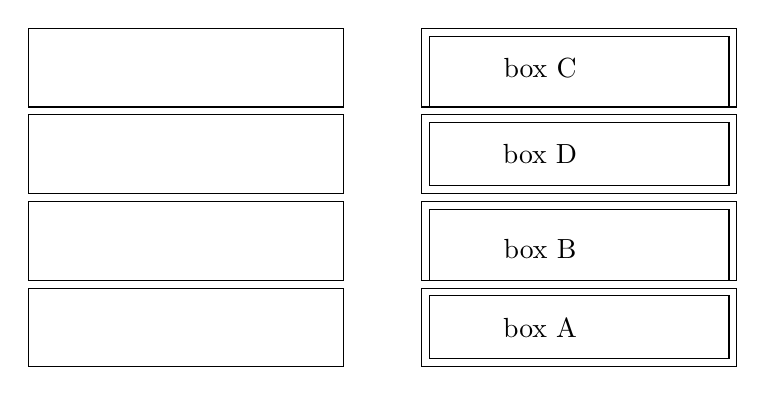
\begin{tikzpicture}
\draw (0,0) rectangle (4,1);
%\draw (0.1,0.1) rectangle (3.9,0.9);
\draw (5,0) rectangle (9,1);
\draw (0, 1.1) rectangle (4,2.1);
%\draw (0.1, 1.2) rectangle (3.9 ,2.0);

\draw (5, 1.1) rectangle (9,2.1);

\draw (0, 2.2) rectangle (4,3.2);
%\draw (0.1, 2.3) rectangle (3.9,3.1);

\draw (5, 2.2) rectangle (9,3.2);

\draw (0, 3.3) rectangle (4,4.3);
%\draw (0.1, 3.4) rectangle (3.9,4.2);

\draw (5, 3.3) rectangle (9,4.3);
\draw (5.1, 0.1) rectangle (8.9,0.9);
\draw (5.1, 1.1) rectangle (8.9,2.0);
\draw (5.1, 2.3) rectangle (8.9,3.1);
\draw (5.1, 3.3) rectangle (8.9,4.2);

\node  at (6.5, 0.5) {box A};
\node  at (6.5, 1.5) {box B};
\node  at (6.5, 2.7) {box D};
\node  at (6.5, 3.8) {box C};


\end{tikzpicture}
\\
\\
\noindent We are now done, since the source bookcase  is empty.
\\
\\
\noindent It is rather  tedious  and wasteful  to draw bookcases  to illustrate the working of the algorithm, so let us introduce a simpler 'tuple' notation for the same example, where we  use ( [source], [dest], n)  as a shorthand, with ',' separating the shelves:
\\
\\
\(   ( [D,C,B,A], [, , , ], 17)    \Rightarrow  pos = 0  \Rightarrow  ( [D,C,B,], [A, , , ], 17)    \)  for step 1
\\
\\
\(  ( [D,C,B,], [A, , , ], 17)     \Rightarrow  pos = 1 \Rightarrow  ( [D,C,,], [A, B, , ], 8)    \) for step 2
\\
\\
\(   ( [D,C,,], [A, B, , ], 8)     \Rightarrow  pos = 2 \Rightarrow  ( [D,,,], [A ,B ,C, ], 2)   \) for step 3
\\
\\
\(  ( [D,,,], [A ,B ,C, ], 2)     \Rightarrow  pos = 2 \Rightarrow  ( [,,,], [A ,B ,D, C ], 0)    \) for step 4
\\
\\
\noindent We also pre-labeled the 'boxes' in the source. We are not using the labels in the algorithm, but they help us to keep track of what is ending up where, along the way. 
\\
\\
Let us try the permutation 10,
\\
\\
\(   ( [D,C,B,A], [, , , ], 10)    \Rightarrow  pos = 0  \Rightarrow  ( [D,C,B,], [A, , , ], 10)    \)  for step 1
\\
\(  ( [D,C,B,], [A, , , ], 10)     \Rightarrow  pos = 0 \Rightarrow  ( [D,C,,], [B, A, , ], 5)    \) for step 2
\\
\(   ( [D,C,,], [B, A, , ], 5)     \Rightarrow  pos = 2 \Rightarrow  ( [D,,,], [B ,A ,C, ], 1)   \) for step 3
\\
\(  ( [D,,,], [B ,A ,C, ], 1)     \Rightarrow  pos = 1 \Rightarrow  ( [,,,], [B ,D, A, C ], 0)    \) for step 4
\\
\\
We can further simplify by leaving out the intermediate steps, now we understand the algorithm
\\
\\
\(   ( [D,C,B,A], [, , , ], 10)    \Rightarrow  ( [,,,], [B ,D, A, C ], 0)    \) 
\newpage

\noindent and furthermore by labelling the boxes with the shelfnumber instead of letters
\\
\\
\(   ( [0,1,2,3], [, , , ], 10)    \Rightarrow  ( [,,,], [2 ,0, 3, 1 ], 0)    \) 
\\
\\
and finally by letting the source be implicit  \( [0,1,2,3,4....,n]  \)  and just specifying the number of the  permutation  and the result: 
\\
\\
\(     10   \Rightarrow  [2 ,0, 3, 1 ]    \) 
\\
\(     17   \Rightarrow  [3 ,2, 0, 1 ]    \) 
\\
\(     0   \Rightarrow  [0 ,1, 2, 3 ]    \) 
\\
\(     23  \Rightarrow  [3 ,2, 1, 0 ]    \) 
\\
\newpage
\noindent
Looking at all  e \(  4!  = 24  \)  permutations shows a systemic pattern  if we delete '0' (the last added item) from the list
\begin{tabbing}
\\
\(     0   \Rightarrow  [0; 1; 2; 3] \)  dele\=ting \=0  gi\=ves  \=\(  [1; 2; 3] \)
\\
\(     1 \Rightarrow  [0; 1; 3; 2] \)   \>-   \> -   \> -  \> \(  [1; 3; 2] \)
\\
\(     2  \Rightarrow  [0; 2; 1; 3]\)   \>-  \>- \>-    \>  \(  [2; 1; 3] \)
\\
\(     3   \Rightarrow  [0; 3; 1; 2] \)  \>-  \>- \>-    \>  \(  [3; 1; 2] \)
\\
\(     4   \Rightarrow  [0; 2; 3; 1] \)  \>-  \>- \>-    \>  \(  [2; 3; 1] \)
\\
\(     5   \Rightarrow  [0; 3; 2; 1] \)  \>-  \>- \>-    \>  \(  [3; 2; 1] \)
\\
\(     6   \Rightarrow  [1; 0; 2; 3] \) \>-  \>- \>-    \>  \(  [1; 2; 3] \)
\\
\(     7   \Rightarrow  [1; 0; 3; 2] \)  \>-   \> -  \> -      \> \(  [1; 3; 2] \)
\\
\(     8   \Rightarrow  [2; 0; 1; 3]\)  \>-  \>- \>-    \>  \(  [2; 1; 3] \)
\\
\(     9   \Rightarrow  [3; 0; 1; 2] \)  \>-  \>- \>-    \>  \(  [3; 1; 2] \)
\\
\(     10   \Rightarrow  [2; 0; 3; 1] \)  \>-  \>- \>-    \>  \(  [2; 3; 1] \)
\\
\(     11   \Rightarrow  [3; 0; 2; 1] \) \>-  \>- \>-    \>  \(  [3; 2; 1] \)
\\
\(     12   \Rightarrow  [1; 2; 0; 3] \)\>-  \>- \>-    \>  \(  [1; 2; 3] \)
\\
\(     13   \Rightarrow  [1; 3; 0; 2] \)\>-       \> -      \> -      \> \(  [1; 3; 2] \)
\\
\(     14   \Rightarrow  [2; 1; 0; 3] \)  \>-  \>- \>-    \>  \(  [2; 1; 3] \)
\\
\(     15   \Rightarrow  [3; 1; 0; 2] \)  \>-  \>- \>-    \>  \(  [3; 1; 2] \)
\\
\(     16   \Rightarrow  [2; 3; 0; 1] \) \>-  \>- \>-    \>  \(  [3; 1; 2] \)
\\
\(     17   \Rightarrow  [3; 2; 0; 1] \) \>-  \>- \>-    \>  \(  [3; 2; 1] \)
\\
\(     18   \Rightarrow  [1; 2; 3; 0] \)\>-  \>- \>-    \>  \(  [1; 2; 3] \)
\\
\(     19   \Rightarrow  [1; 3; 2; 0] \)\>-   \> -  \> -  \> \(  [1; 3; 2] \)
\\
\(     20   \Rightarrow  [2; 1; 3; 0] \)  \>-  \>- \>-    \>  \(  [2; 1; 3] \)
\\
\(     21   \Rightarrow  [3; 1; 2; 0] \)  \>-  \>- \>-    \>  \(  [3; 1; 2] \)
\\
\(     22   \Rightarrow  [2; 3; 1; 0] \) \>-  \>- \>-    \>  \(  [2; 3; 1] \)
\\
\(     23   \Rightarrow  [3; 2; 1; 0] \)\>-  \>- \>-    \>  \(  [3; 2; 1] \)
\\
\end{tabbing}
\noindent
we notice four repetitions of the same  \( 6 = 3!  \)  lines, which are all  the permutations of \( [ 1; 2; 3] \)  The four is explained by the ways it is possible to extend the list with a 0 in four different positions.  
\\
\\
This gives us a clue to how to find the n leading to a given permuation.
\newpage
\section{Finding n from the permutation}
\text
Given a permutation p  of [0,1,2,3,4,.....n-1] the n, which produced it, is given  by 
\[  
n(p) = \sum_{i = 0}^{n-2} F(i,p)
\]
\\
\begin{tabbing}

where\=
\\
\\
   \> \(  F(i,p) =  pos( i,  p_{i} )  \times (( | p_{i} |  - 1 )!)   \)
\\
\\
 \>  \(   pos( i,  p_{i} | )  \) is the position  of  i in  \(  p_{i} , 0,1,2 ....    \) 
\\
\\
       \>    \( p_{i}  \)  is p with all values less than i removed, hence  \( p_{0}  = p     \) 
\\
\\
    \>  \(  | p_{i} | \) is the length of  \(  p_{i}     \)  
\\
\\
  \>  \(  x!   \)  is the faculty of x, \( x!  = x \times   (x-1) \times   (x-2) \times ....  \times 2 \times 1 \)
\\
\\
For our previous \=example, \=   \(   [3 ,2, 0, 1 ]  \)   we get
\\
\\
\> \( pos(0,[3,2,0,1) \times ( |   [3 ,2, 0, 1 ] |-1) ! \)
\\
\>+   \(  pos(1,[3,2,1) \times ( |   [3 ,2, 1 ] |-1)!  \)
\\
\>+  \( pos(2,[3,2) \times ( |   [3 ,2,  ] |-1)  !  \) 
\\
\\
which equals \>  \(   ( 2 \times 6 ) + (2  \times 2 ) + ( 1 \times  1) =  12 +4 +1 = 17    \)
\end{tabbing}

\section{finding the inverse permutation}
\text
Given a permutation of   \(  [ 0, 1, 2, 3] \) to \(  [3, 0, 2, 1] \)  we can try to find the n corresponding to the  inverse permuation.
\\
\\
The nverse permuation should  move position 1 to  position 0, postion 3 to  position 1, position 2 to  position 2 and position 0 to  position 3 , 
meaning the inverse permutation is [1,3,2,0]  and using the result from the previous section
\\
this means \( n = 3 \times 6 +  0 \times 2 + 1 \times 1 = 19 \)
\\
\\
\begin{tabbing}
As a formula \= the inverse permutation to P (from \(  [0,1,2,3.....,n-1] \) , which we call  \( P^{-1} \) , 
\\
is,  using the pos(i, p) function from the previous section :
\\
\\
\> \( P^{-1} =  [ pos(0,P); pos(1;P); pos(2,P),......,pos(n-1,P)] \)
\end{tabbing}
\newpage 
  \section{python Code} % creates a section
\begin{lstlisting}
def myPerm( N1, ain):  
	   return my_Perm(N1, ain.copy() )
	   
def my_Perm(N2, ain ):
		n1 = N2
		res = []
		for n in range( 0, len(ain) ):
			res.insert(n1 % (n+1), ain.pop())
			n1 = n1 // (n+1)
		return res

def findN(aPermutation) :
    return _findN(aPermutation.copy(), 0)
			
def _findN(aPerm, ll) :
    alen = len(aPerm);
    match alen :
      case 0: 
         return 0;	  		
      case 1:	
         return 0;
      case 2:	
         if( (aPerm[0]) == 0):
            return ll
         else:
            return ll+1	  				
      case _:	
         pos = find0(aPerm)
         fac_alen_minus_1 = math.factorial(alen-1)
         aPerm_ = remove0(aPerm.copy())
         return _findN( aPerm_, ll + ( pos * fac_alen_minus_1))

def Pos( N, aPerm):
    for n in range( 0, len(aPerm) ):
       if( aPerm[n] == N):
            return n
    return -1 
    
def Inverse( aPerm ):
    res = [];
    for n in range( 0,  len(aPerm)):
         res.append( Pos(n, aPerm)) 	  
    return res
\end{lstlisting}
\newpage

  \section{C++ Code} % creates a section
\begin{lstlisting}
void MakePermutation(u64 index,
			const  std::vector<Something>& src, 
			std::vector<Something>& dst)
 {
  u64 n1 = index;
  u64 pos = 0;
  uint counter = 0;
  dst.clear();

   for (int ix = src.size() ; ix > 0; ix--) {
 	pos = n1 % (counter + 1);
	n1 = n1 / (counter + 1);
	counter++;
	if (pos == dst.size())
		dst.push_back(src[ix-1]);
	else {
		dst.push_back(dst.back());
		for (int i = dst.size()-2; i > pos; i--) dst[i] = dst[i -1];
		dst[pos] = src[ix-1];
	}
   }
}
\end{lstlisting}
\newpage

  \section{Ocaml Code} % creates a section

\begin{lstlisting}
       
let rec 
    (*   insert a at pos in l  *)
      insertAux a pos l acc =  
          if (pos = 0) then (( List.rev acc) @ a::l )      
                               else insertAux a (pos -1) (List.tl l)  ((List.hd l )::acc)
   and
	insert a pos l =  if( pos = 0) then a::l  else insertAux a  pos  l []
   and   
      permuteAux   li n   acc =
      match li with 
      |  [] -> List.rev acc
      | hd::tl  -> 
      let  p = (List.length acc) 
           in let pos = ( n mod (p+1))
           in let n1 = (n / (p+1)) 
           in permuteAux tl n1 (insert hd pos acc)
    and
     (*   the nth permutation of li ( 0 is the null permutation *)
      permute li n =
      match li with 
      | []  -> []         (* empty list*)
      | hd::[] ->  [hd]   (* one element *)
      | hd::tl ->  permuteAux tl n [hd] (* more than one element list*)

let rec find0 alist =  
        find0aux alist 0 
		and
		    find0aux alist count =
          match alist with
          | []  -> -1
          | hd::tl -> if (hd = 0 ) 
                      then  count
                      else find0aux tl (count+1)
 
 let rec remove0aux  alist acc =
 		 match alist with 
 		 | []  -> List.rev acc
 		 | hd::tl -> if (hd = 0)
 		             then remove0aux tl acc
 		             else remove0aux tl ((hd - 1)::acc)
 
let remove0 alist = remove0aux alist []

let rec fac len res =
           if(len <= 0) 
           then res
           else fac (len-1) (len *res)

let rec findNaux alist ll   =
        match alist with
        | [] -> 0
        | [0] -> 0
        | [0;1] -> ll
        | [1;0] -> (ll+1)
        |  _    -> 
                let pos = find0 alist in
        				let alen = (List.length alist) in
                findNaux (remove0 alist) (ll + pos * (fac (alen - 1) 1)  )

let rec findN alist = findNaux alist  0 ;;

let rec pos1 ix alist counter =
       match alist with 
       | [] ->  -1
       | hd::tl -> if( ix = hd) 
             then counter
             else pos1 ix tl (counter+1)

let rec pos ix alist = pos1 ix alist 0
     
let rec findInverse1 alist blist ix acc =
	 match alist with
	 | [] -> List.rev acc 
	 | ahd::atl -> findInverse1 atl blist (ix+1) ( (pos ix blist)::acc)
					 
let rec findInverse alist =
	 findInverse1 alist alist 0 [] 
					 
\end{lstlisting}

\newpage
 \section{Ocaml Code using pInt( large integers) } % creates a section
\begin{lstlisting}

let rec facultAux a acc =
   if(isZero a) then acc else  facultAux (sub a (fromInt 1)) (schoolbookMul a acc);;
   
let facult a = facultAux (fromInt a ) (fromInt 1);;

let rec 
(*   insert a at pos in l  *)
      insertAux a pos l acc =  
      match l with 
      | [] -> if (pos = 0) 
              then List.rev ( a::acc) 
              else List.rev acc 
      | hd::tl -> if (pos = 0) 
               then insertAux a (pos - 1) l  (a::acc)
               else insertAux a (pos - 1) tl (hd::acc)
   and
       insert a pos l =   insertAux a  pos  l  []
   and   
      permuteAux   li n   acc =
      match li with 
      |  [] -> acc
      | hd::tl  -> 
      let  p = 1+ (List.length acc) 
           in let ( n1, pos)  = quotRem ( fromInt p ) n
           in permuteAux tl n1 (insert hd ( toInt pos ) acc)
    and
    (*   the nth permutation of li ( 0 is the null permutation *)
      permutation rli n =
      let li= List.rev rli in
      match li with 
      | []  -> []         (* empty list*)
      | hd::[] ->  [hd]   (* one element *)
      | hd::tl ->  permuteAux tl n [hd] (* more than one element list*)
\end{lstlisting}
\newpage
\begin{lstlisting}
let rec find0 alist =  
	     find0aux alist 0 
	and
	     find0aux alist count =
	          match alist with
	          | []  -> -1
         		| hd::tl -> if (hd = 0 ) 
                     		 then  count
	                      else find0aux tl (count+1)
 
 let rec remove0aux  alist acc =
 		 match alist with 
 		 | []  -> List.rev acc
 		 | hd::tl -> if (hd = 0)
 		             then remove0aux tl acc
 		             else remove0aux tl ((hd - 1)::acc)
 
 let remove0 alist = remove0aux alist []
        
let rec findNaux alist ll =
        match alist with
        | [] -> []
        | [_] -> []
        | [0;1] -> ll 
        | [1;0] -> (addInt ll 1) 
        |  _    -> 
                let pos = fromInt (find0 alist) in
                let _alen = List.length alist in
        				let fac_alen_minusOne = facult (_alen - 1)  in   
			 					findNaux (remove0 alist)  (add (mul pos fac_alen_minusOne) ll) 

let rec findN alist = findNaux alist  (fromInt 0 )     
		
			 
\end{lstlisting}
       
\newpage

  \section{A larger Python example, a deck of cards} % creates a section
\begin{lstlisting}

import math
import random

def my_Perm(N2, ain ):
	a = ain.copy()  # we don't like functions modifying their arguments
	n1 = N2
	res = []
	for n in range( 0, len(a) ):
		res.insert(n1 % (n+1), a.pop())
		n1 = n1 // (n+1)
	return res

# make a deck of cards
def makedeck():
	res = []
	for colour in [ "Hearts", "Spades", "Diamonds", "Clubs" ]:
		for rank  in ["Ace", "2", "3", "4",
                       "5", "6","7", "8", 
                        "9", "10", "Jack", 
                        "Queen", "King" ]:
			res.insert(0, rank + " " + colour )
	return res

deck = makedeck()  #make a deck sorted by suit

# shuffle  a new deck of cards
def shuffle():
	return   my_Perm( random.randrange(0,math.factorial(52)), makedeck())	

# re-shuffle a deck of cards
def reshuffle( adeck):
	return   my_Perm( random.randrange(0,math.factorial(52)), adeck)	

#deal four hands of 13 cards
def dealHands (adeck):
	res = []
	res.insert(0,adeck[0:13])	
	res.insert(0,adeck[13:26])	
	res.insert(0,adeck[26:39])	
	res.insert(0,adeck[39:52])
	return res	

#  print the four hands
def printHands( hands):
	print( hands[0])
	print( hands[1])
	print( hands[2])
	print( hands[3])
		

\end{lstlisting}
\newpage


\end{document} % This is the end of the document